%This research paper---as opposed to a “narrative/composition” paper (e.g., for an English course)---is a written report based on a systematic analysis that you conduct on a topic concerning Complexity Theory in the Social Sciences. Your analysis will apply a selection of concepts, theories, models, or other ideas covered in this course. The actual analysis comes first; the paper comes second, so think of this paper as a “lab report:” you write it up after you have conducted your experiment. Do not begin writing this paper before you have finished (or almost finished) your analysis, otherwise you will likely encounter serious problems. As a general guideline, papers like this are usually 15-20 pages in length. Double-space the entire paper, except the Bibliography.
%
%Use any major citation style (Turabian, MLA, Chicago); just be consistent throughout.
%
%Use any major citation style (Turabian, MLA, Chicago); just be consistent throughout.
\documentclass[pdftex,12pt,oribibl]{llncs}
\usepackage[american]{babel}
\usepackage{wrapfig}
% \newcommand{\x}[1]{ }
% This is where the bibliography stuff needs to happen
%\usepackage[style=apa, backend=biber]{biblatex}
%\DeclareLanguageMapping{english}{american-apa}
\usepackage{biblatex}
\addbibresource{billTolls.bib}
%\addbibresource{Projects-garbageCanCongress.bib}
\usepackage[utf8]{inputenc}
\usepackage{csquotes} % context sensitive quotes ---makes this look good
\usepackage[pdftex]{graphicx}
\usepackage{xfrac}
\usepackage{cleveref}

\begin{document}

%\title{For Whom the Bill Tolls}
%\subtitle{Policy Formation through Simulated Annealing }
\title{A Model of Policy Formation through Simulated Annealing:}
\subtitle{The Impact of Preference Alignment on Productivity and Satisfaction}
\titlerunning{Policy Formation through Simulated Annealing}
\author{Scott Atherley \and Clarence Dillon \and Vince Kane}
\institute{George Mason University\\
\thanks{We wish to thank Maksim Tsvetovat who introduced us to applications of simulated annealing to Organizational Theory and inspired us to extend it, adapt it, and to think about organizations and processes where it seems to fit especially well.  We also thank an anonymous reviewer for helpful feedback provided on a previous draft of this paper.}
\email{\{satherle, cdillon2, vkane2\}@gmu.edu}}

\maketitle

%Cover page: Title, Your Name, ID, Course name, Date, and Abstract ( < 200 words).
%Title: Descriptive, well-focused, and brief. Use a subtitle to provide more information. Some hypothetical examples: “Power Law Analysis of Wealth in Ireland and Peru: A Comparative Analysis”; “Scaling in the International Airline Network“, “Governmental Capacity and Criticality in Domestic Political Instability”; “Comparing Estimates of the Pareto Exponent”. Pick a tentative title first.
%
%Do not settle on a final title until your paper is completely finished.
%

\begin{abstract}
 We are interested in how preference correlations can impact policy-maker productivity and their satisfaction with resultant policy. 
 We applied a simulated annealing process as a model of revising draft legislation in peer and committee reviews before submission to a floor vote.
 Results indicate that having exogenous, common issue priorities is required for productivity but that some structures inhibit productivity, particularly where preference schedules are uncorrelated.
 Our model also demonstrates lower system efficiency, and lower overall satisfaction, as policy is negotiated through compromise to achieve higher production.\\
 
 \textbf{Key words}: simulated annealing $\cdot$ policy formation $\cdot$ organizational theory $\cdot$ preference alignment $\cdot$ network structure
\end{abstract}

\section{Introduction}
%(approximately .5 pages) Write this section last!
%A common (bad) idea is to begin by writing this section first—it just doesn’t work because it tends to get too long and disconnected from core results. Introduce the topic of your research and its motivation. Address these questions:
%
%What is the main topic?
%
%Why is it important?
%
%What do some existing works (from readings and your own background bibliographic research) say about this topic?
%
%Conclude this section with a summary paragraph stating (one sentence each):
%the specific topic;
%main hypothesis examined in your analysis;
%approach used for this study;
%major finding. Use boldface each time you use a course term for the first time (e.g., Pareto exponent, criticality, heavy tail, exponential distribution, etc.).

It is a trope of Western democratic ideals that a democracy---govern-\\ance by vote---produces the greatest happiness for its citizenry, or the least unhappiness for a majority of it.
%On the other hand, we also suspect that as a policy-making system, it is highly inefficient and -- in the extreme -- unproductive.
Our intuition is that diversity and divides in policy preferences can result in legislative deadlock and lower overall satisfaction with legislative outcomes.
We were motivated to this research wanting to understand why the $113^{th}$ U.S. Congress was particularly unproductive.
Political science often models congressional ideology backward from voting decisions \parencite{m74, k89}, party influence \parencite{cm93,cm05,a95,k91, k98}, and committee dynamics \parencite{sw87, gk89, m04}.
Our research complements other studies by developing a computational model of policy development through draft legislation, working forward from arbitrary ideological foundations.
Viewing bill revision as a process that optimizes legislative body satisfaction within a system of competing legislator preferences, we judged simulated annealing (SA, hereafter) to be the non-deterministic optimization method most suited for modeling this.

As a generalized model of policy-making, the results are broadly applicable to a wide range of policy-making organizations: legislative bodies at the national or local level, regulatory bodies, standards organizations, and conference committees, for example.

Our simulation model enables quantitative analysis of the productivity and satisfaction of three typified legislatures: with unified, bi-modal (bipartisan), or completely uncorrelated sets of preferences. 
Results indicate that party partisanship alone does not explain a Congress's inability to produce legislation.

\section{Model and Methods}
%(3-4 pages) Write this section third!
%
%This section identifies and defines those concepts, models, theories, or other course ideas and tools that you used in order to carry out your analysis. Which concepts, data, theories, principles or other analytical tools from the course—from lectures or readings—did you use in this study? Which sources?
%
%Which data processing procedures? Which cases or samples? Which time periods (epochs)? Key:reproducibility! I must be able to replicate your findings, based on the information provided in this section.

\subsection{Model Overview}
In this section, we describe implementation of a model of policy formation through simulated annealing.
We initialize each case by generating a legislature and its internal social network. 
Legislators have preferences on a set of issues, prioritizing some issues over others.
They take turns sponsoring bills, which get reviewed and revised through two rounds of SA before the entire legislative body votes on the bill.
We captured productivity, satisfaction, and amount of compromise as the relevant metrics for each simulation run.
We describe the initialization and simulation processes and experimentation methods in more detail below.
\footnote{In the interest of brevity, we have omitted some detail descriptions of the initialization and simulation; however, these details,as well as the model itself, may be found in the online supplement at https://github.com/strangeintp/garbage-can-congress/wiki}.

\subsection{Model Initialization}
The first step in the simulation initializes the model by generating a \texttt{State} object, which realizes the parameters of that run scenario: a heterogeneous set of 100 legislators, each with priority-ranked positions on a set of 75 issues, assigned stochastically but correlated through State- and party-provided seed vectors. 
The \texttt{State} object then organizes the legislators into a social network making a realistic number of connections between the most similar legislators.

\subsubsection{Initializing the Model Environment}
For our model, we assume that several core issues represent powerful, crystallizing factors that differentiate our simulated parties.
Thus, party ``platforms'' consist of vectors of positions and priorities on a set of issues that includes both \texttt{State\_Priorities} and a random sample of high-priority \texttt{Ideology\_Issues}.
These vectors are used as ``seeds'' for the stochastic generation of individual legislator preferences.
\subsubsection{Legislator Initialization}
Each legislator's issue priorities are assigned with a stochastic preferential attachment method to the seed values provided by the \texttt{State} object.
This generates a power law distribution of priorities for that legislator and provides some correlation in legislator priorities to the extent that seed vectors are similar (as determined by state priorities and party ideology).

We assume that party-affiliated legislators adopt the positions of their party; for all other issues (and all issues for unaffiliated legislators), positions are assigned uniform randomly from the range of allowed position values ($2^4$ for our model).
The end-result of this process is a set of legislator agents with heterogeneous but correlated policy preferences as conditioned by party ideologies and state priorities, and with the strength of correlation determined by party-alignment.
\subsubsection{Network Generation}
The final step of initialization generates a social network, using both homophily \parencite{msc01, br11} and preferential attachment \parencite{Barabasi1999}, based on preferences assigned in the previous step. 
Preferential attachment is as described in Barabasi and Albert (1999), with $m=5$ new edges selected randomly from a \textit{pdf} distribution of degree in the sub-network of potential allies of each legislator. 
The set of potential allies is selected using a preference-weighted likelihood over all issues.
The typical outcome of this procedure is a network among legislator agents with ``small-world'' properties \parencite{Watts1998}, consistent with existing research on social networks in the U.S. Congress \parencite{Granovetter1978} \footnote{We verify ``small-worldness'' of the networks produced by the model using the Humphries and Gurney metrics \parencite{hg08}.}.
\subsection{Simulation Algorithm Overview}
Having defined a population of legislators and their relationship to each-other, we next establish a procedure for legislators to engage in the business of law-making.\footnote{One might argue that this is a departure from realism, as the current Congress does not appear to do this.
However, we are attempting to generalize a model of law-making in legislatures.
Some legislatures do periodically legislate.}
In our model of law-making, the simulation sequentially repeats the following process for 200 proposals (or halts if all issues are passed into law):
\begin{enumerate}
\item Proposal:
\begin{enumerate}
\item A random legislator is chosen to sponsor a bill.
\item The sponsor proposes a draft bill on any issue that has not already been addressed by law. This initial draft reflects the sponsor's position on that issue.
\end{enumerate}
\item Draft circulation among cosponsors:
\begin{enumerate}
\item All legislators connected to the sponsor in the social network are selected as cosponsors.
\item The cosponsors revise the draft using SA; new issues may be added to the bill during the revision process and solutions on existing issues may change.
\end{enumerate}
\item Committee review:
\begin{enumerate}
\item The draft is referred to a committee, reflecting committee agenda-setting powers \parencite{cm93, cm05}.
Legislators for whom the main issue of the bill is a high priority are assigned to the relevant committee.
\item The committee revises the bill by SA; again, new issues may be added and existing solutions changed.
\end{enumerate}
\item Floor vote:
\begin{enumerate}
\item The bill is referred to the floor for a vote.
\item A legislator votes `yes' to a bill when her satisfaction with it is greater than the model parameter \texttt{satisfaction\_threshold}.
\item If the bill passes by simple majority (\textgreater 50\% votes), the bill is made into law; \textit{i.e.}, the solutions addressed by the bill are recorded and the issues may not be revisited for the remainder of the realization.
\end{enumerate}
\end{enumerate}
\subsubsection{Simulated Annealing}
Bill revision is implemented by the Metropolis algorithm for simulated annealing \parencite{mrrt53, kgv}.
Our energy function is the cumulative dissatisfaction of all reviewers over all dimensions of the bill. Increases of $0.1$ in dissatisfaction were accepted with probability \sfrac{1}{2} at the maximum temperature.
Higher satisfaction energy states are automatically accepted.
\footnote{The online supplement provides more detail.}
\subsection{Model Calibration}
We calibrated legislators' \textit{satisfaction thresholds}---the point at which they vote ``yes'' on legislation---to achieve a ~4\% pass-rate, comparable to passage rates in the actual US Congress (between 2\% and 7\% in recent history).\footnote{Pass rates are equal to the total number of bills passed in a given Congress divided by the total counts of introduced legislation for that Congress. Data to calculate pass rates was collected from Civic Impulse LLC (http://www.govtrack.us).\label{passfn}}
\subsection{Experiments}
Table \ref{params} identifies key parameters used in the model for the suite of experiments.
The experiment suite was designed factorially, exercising all combinations of values shown in the table -- excepting \texttt{Green\_Fraction} variation when {\texttt{Unaffilitated\_Fraction} = 1.0}, which is a degenerate case -- resulting in 28 unique experiments.
30 simulations were realized per experiment.

For each realization, we recorded: the number of laws passed, the number of issues addressed by law (i.e. provisions), and legislative body satisfactions over all bills before and after SA revisions. 
To keep the data set manageable, we recorded a sample run history for only a single realization of each experiment.
Aggregate statistics (averages and standard deviations) were also calculated and recorded for the output metrics of all realizations of an experiment.


\begin{table}[htp]
 \caption{Simulation Parameter Space}
 \begin{tabular}{lp{2.25in}c}
 \hline\noalign{\smallskip}
 Parameter & Description & Value [Variation] \\
 \noalign{\smallskip}
 \hline
 \noalign{\smallskip}
 \texttt{Unaffilitated\_Fraction} & Fraction of the legislative population with no ideological party  affiliation. & [0.05, 0.5, 1.0] \\
 \texttt{Green\_Fraction} & Fraction of the party-affiliated population belonging to the \textit{Green} party. Remainder belong to the Yellow party. & [0.5, 0.75, 1.0] \\
 \texttt{Ideology\_Issues} & Ideological platform issues for the parties. & [0, 5] \\
 \texttt{State\_Priorities} & High-priority issues for all legislators, regardless of affiliation. & [0, 5] \\
 \hline
 \end{tabular}
 \label{params}
\end{table}


\section{Results and Findings}
%(2 pages) Write this section first!
%
%Present your results of analysis in this section. 
Fourteen of the 28 experiment combinations were uniformly unproductive (produced no laws), as follows:
\begin{enumerate}
\item All four cases with no party structure,
\item Scenarios with 50\% unaffiliated, 25\% Green, and 25\% Yellow,
\item Scenarios with no external priorities (an additional 5), and
\item One case with 5\% unaffiliated members, 50\% Green members, and no ideology-based priorities.
\end{enumerate}
For the remaining productive cases, Figure \ref{combined} presents run results across the three aggregate metrics captured for each run (total satisfaction and number of laws passed, plotted against number of provisions added.) 

\begin{figure}[h!]
\centering
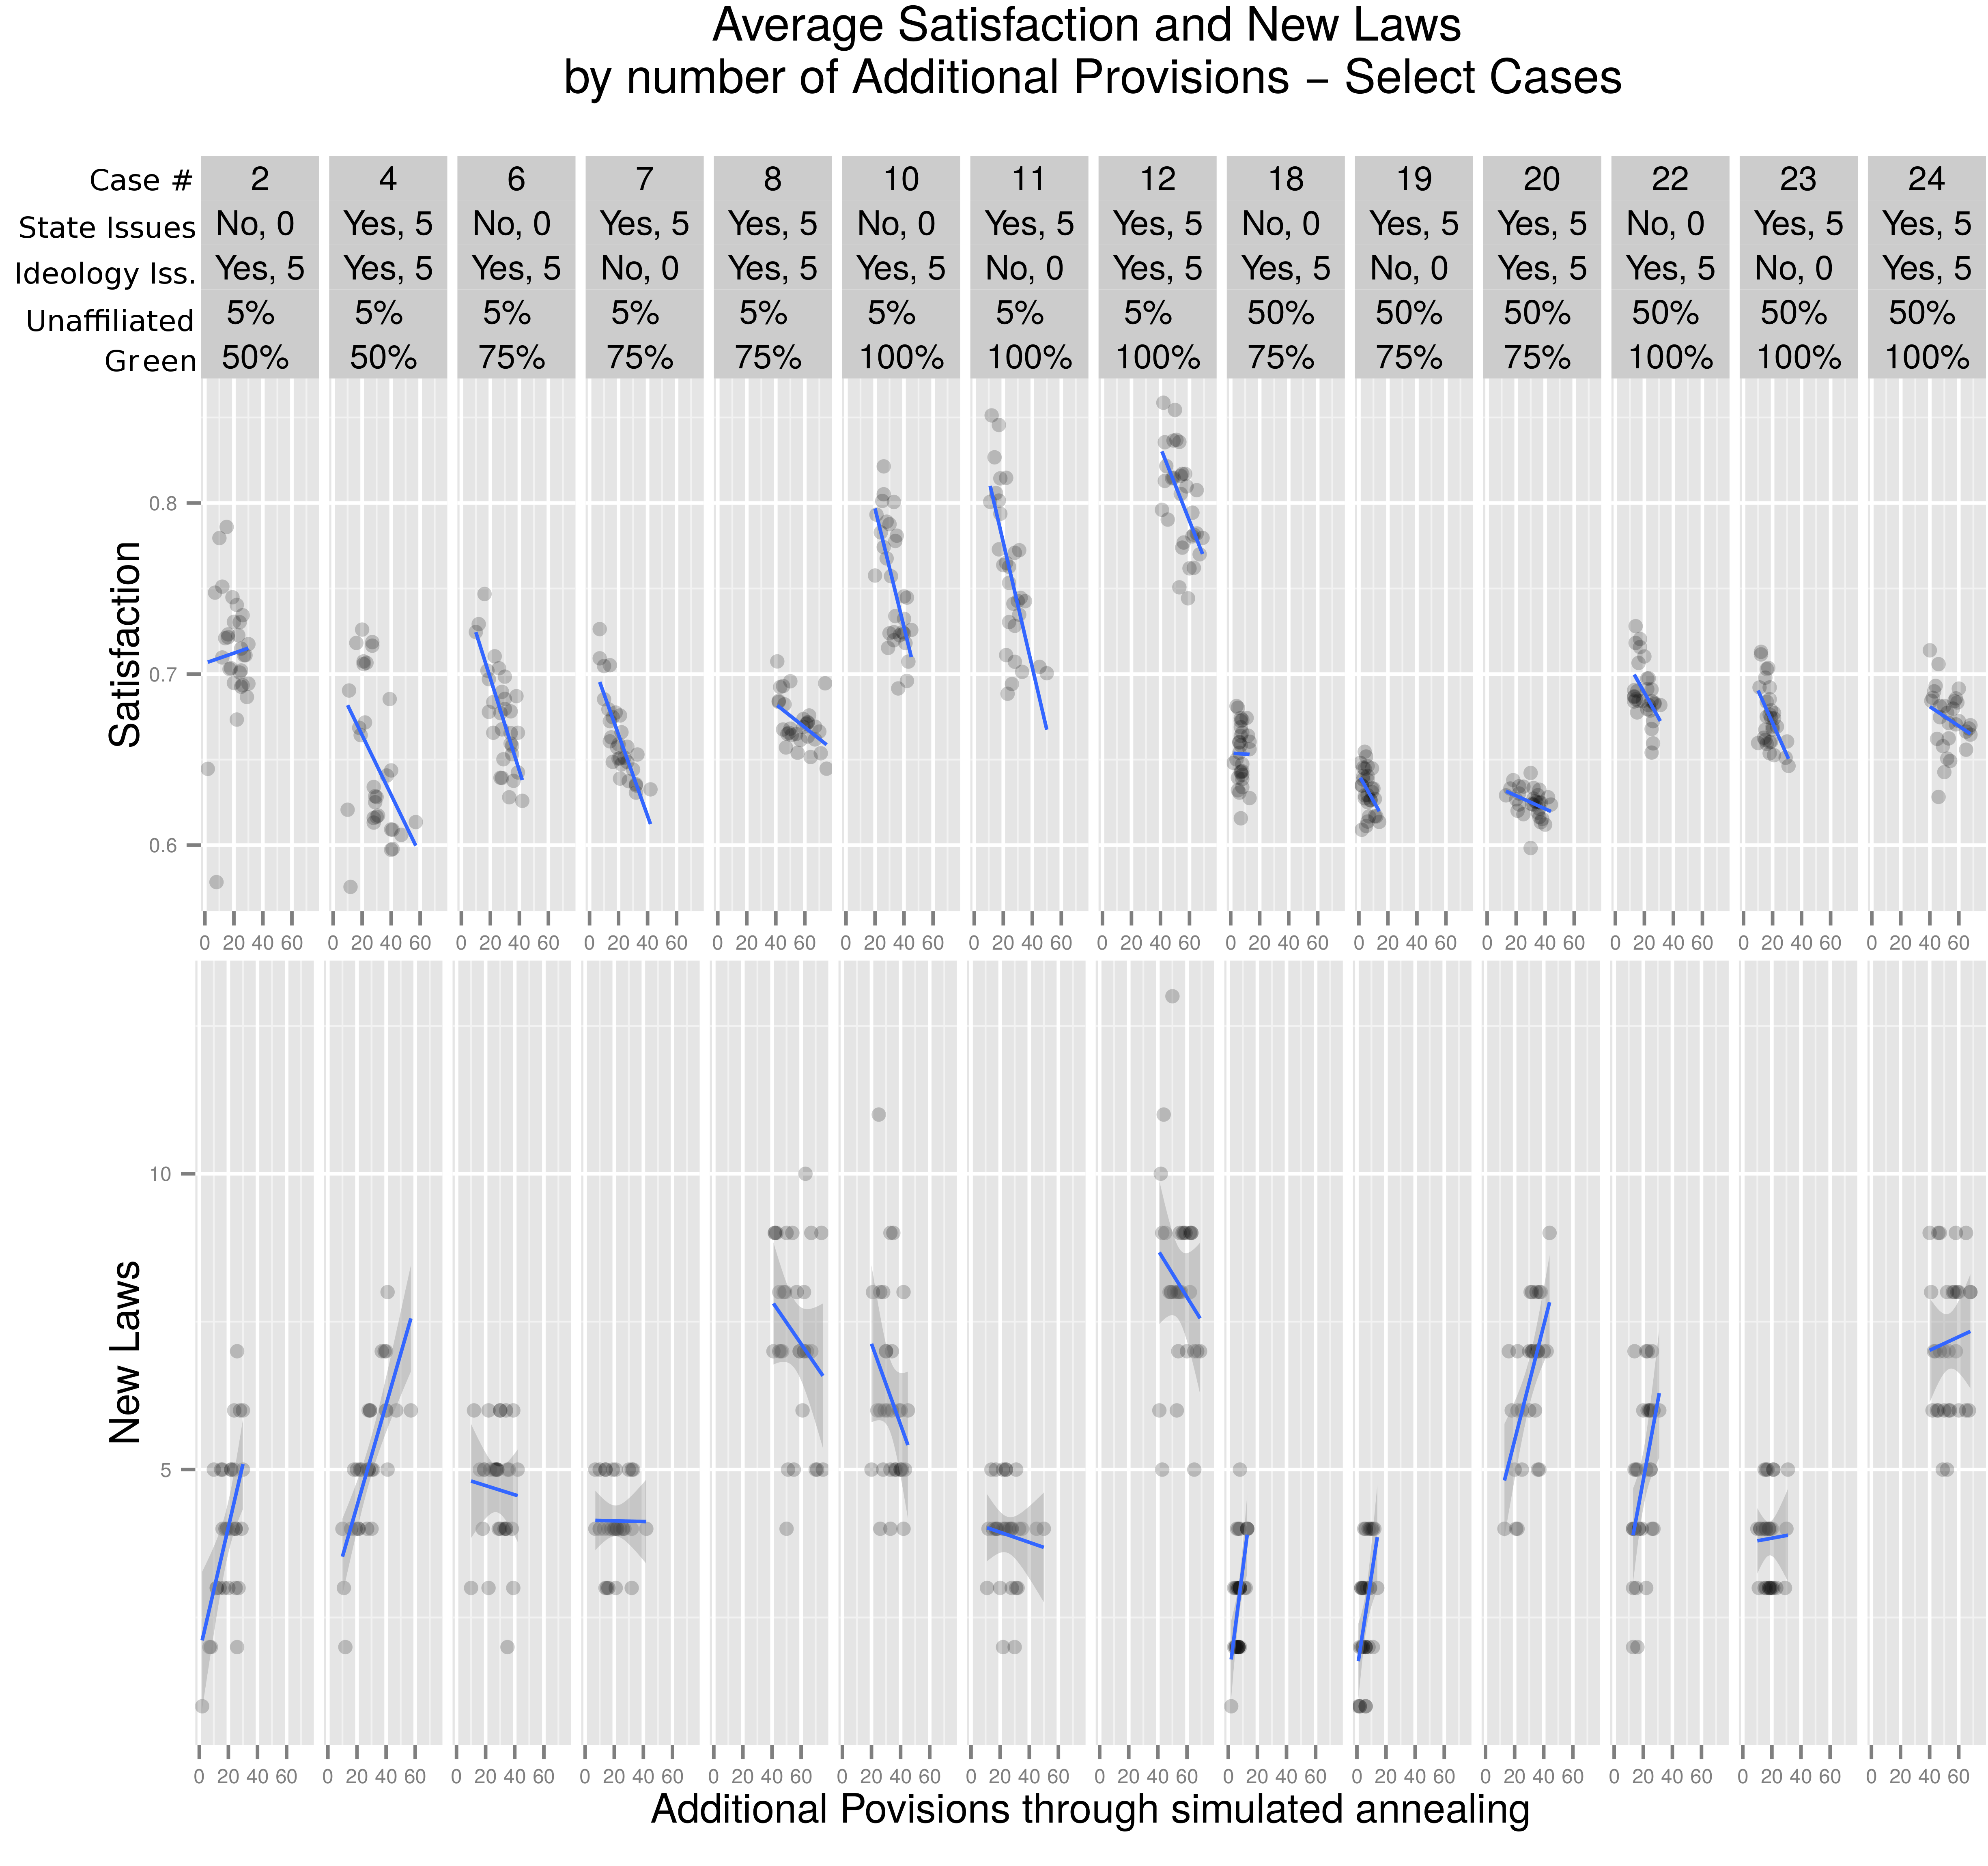
\includegraphics[width=4.75in]{combinedResults.png}
\caption[ ]{Experiment suite results for productive scenarios.  The trend lines indicate a best fit linear correlation to the number of additional provisions.} 
\label{combined}
\end{figure}

%What did your analysis reveal?
%What did the ideas identified in the previous section show you when applied to the topic of your research?
%State your findings using vocabulary learned in the course.
%Imagine making an oral presentation of your main findings or results.
%State your first main finding or result. Then the second, and so on. You may
%want to include graphs, maps, tables, chronologies, diagrams, etc. to support your
%analysis. Label each item.
Interpreting these results, our main findings are:
\begin{enumerate}
\item Higher correlation of preferences results in higher productivity.
\item Higher productivity requires increased provisions.
\item Partisanship is not necessarily an impediment to productivity (see cases 2 and 4).
\item Bipartisan networks (even division of party-affiliated legislators) with more external priorities can be more productive than majorities or super-majorities (with fewer external priorities).  Compare case 4 to cases 11, 18, 19, and 23.
\item Despite higher productivity, overall satisfaction decreases with increased provisions (note negative trend lines in the ``Satisfaction'' row of Figure \ref{combined}).
\end{enumerate}

\section{Discussion}
%(3 pages including tables, figures) Write this section second!
%
%This section is entirely based on section 3.
Based on our results and findings, we can generalize about the importance of having external priorities for self-tasking organizations, such as the U.S. Congress, that undertake complex tasks (law generation) requiring group approval.\footnote{Note that production of an academic paper with multiple authors may fit this generalized formulation, as well.}
Having at least some priorities established externally seems to be required for self-tasking organizations to be productive. 
As a rule, the cases with more externally-defined priorities are more productive than the cases with fewer externally-defined priorities. 
The cases with no externally-defined priorities were consistently unproductive. 
It is tempting to say that this points at the role of leadership---both from within organizations (ideology issues) and from above them (state priorities)---but this will be a question for future research.

Our initial motivation for this research was consideration of the common assertion that a dysfunctional Congress (if measured by ability to pass law) is caused by tensions between the two major political parties in the U.S.
Our results -- in particular, findings 3 and 4 -- do not support the assertion that polarization of preferences alone leads to an unproductive legislature; other factors such as manipulation of the political process are more likely causal.

Finding \#2 demonstrates that higher productivity requires increased provisions.
In a legislative context, these provisions (or ``riders'') represent effort diverted to individual interests that are not [necessarily] focused on the task at hand.
These riders are commonly recognized as the ``cost of doing business''.
Abstracting from a legislative context, we may generalize by saying that higher productivity comes with the cost of lower system efficiency.

Finally, finding \#5---that satisfaction decreases with increasing provisions---captures the social aspects of negotiation and compromise.  
In other words, policy makers are willing to cede adverse positions on their lower-priority issues as a cost of attaining higher satisfaction with the total law, and total satisfaction decreases as these issues are added. 
Conversely, bills start off in a low-satisfaction state and gather provisions as a way of garnering votes.  
In either case, more issues are needed to retain or attain sufficient satisfaction to pass new legislation.
\subsection{Implications for future research}
%How would you conduct a follow-up study?
%Would you do things differently?
%How so?
Further research might vary the network-structure generating parameters with finer resolution to identify the tipping points in the outcomes:
How much of a majority is needed for compromise to yield satisfaction and productivity? 
How much leadership intervention (ideology) is required to overcome inherently unproductive structures?  
How many state priorities are required to ensure sufficient preference correlation, for a given legislature?

We are also interested in understanding the effects of party affiliation on proposals and productivity. This paper reviewed aggregate results from our experiments with the model.
The model could be extended to produce additional detail data about how much compromise is needed, given the characteristics of a bill's sponsor.
We suspect that the sponsor's peer network, if they are in the minority, may modify an otherwise popular proposal with unpopular issues, such that it fails to garner votes at the committee or floor. 
If a bill's sponsor were to intentionally include members from the majority party, or conversely, exclude close connections who may be adverse to a proposal, the annealing process might produce more laws.

\section{Summary}
%(<0.5 pages)
%State the main problem or puzzle that motivated this investigation.
%State your major finding
%State your major implication
%\newpage
We modeled policy-making as a simulated annealing algorithm to find solutions in a complex problem space with interdependent constraints.
We chose the U.S. Congress and legislative process as a case study, but this research may be applied to other policy-making organizations.
Results indicate that partisanship alone is not necessarily an impediment to productivity, provided that there is sufficient alignment of priorities and preferences.
However, higher productivity comes at the cost of lower satisfaction and system efficiency.
We conclude that simulated annealing is a useful method for computationally modeling policy-making, and recommend it for other research projects.
 
%\begin{thebibliography}{}
%
%@book{aw12,
%author = {Adler, Scott and Wilkerson, John},
%publisher = {Cambridge University Press},
%title = {Congress and the Politics of Problem Solving},
%year = {2012},
%}
%
%@book{a95,
%address = {Chicago},
%author = {Aldrich, John},
%publisher = {University of  Press},
%title = {Why Parties?},
%year = {1995},
%}
%
%@book{bj93,
%address = {Chicago},
%author = {Baumgartner, Frank and Bryan Jones},
%publisher = {University of  Press},
%title = {Agendas and Instability in American Politics},
%year = {1993},
%}
%
%@article{b48,
%address = {Chicago},
%author = {Black, Duncan},
%journal = {Journal of Political Economy},
%number = {23–34},
%title = {On the Rationale of Group Decision-making},
%volume = {56},
%year = {1948},
%}
%
%
%@article{br11,
%author = {Bratton, Kathleen and Rouse, Stella},
%journal = {Legislative Studies Quarterly},
%number = {3},
%title = {Networks in the Legislative Arena: How Group Dynamics Affect Co-Sponsorship},
%volume = {36},
%year = {2011},
%}
%
%@article{bhh14,
%author = {Butts, Carter T. and Mark S. Handcock and David R. Hunter},
%journal = {R package version 1.9.0. Irvine, CA},
%title = {network: Classes for Relational Data},
%year = {2014},
%url = {http://statnet.org/},
%}
%
%@article{b08,
%author = {Butts, Carter T.},
%journal = {Journal of Statistical Software},
%number = {2},
%title = {network: a Package for Managing Relational Data in R},
%volume = {24},
%year = {2008},
%}
%
%@book{cff87,
%author = {Cain, Bruce and Ferejohn, John and Fiorina, Morris},
%title = {The Personal Vote},
%year = {1987},
%}
%
%@book{cm93,
%author = {Cox, Gary W. and McCubbins, Mathew},
%publisher = {University of California Press},
%title = {Legislative Leviathan: Party Government in the House},
%year = {1993},
%}
%
%@book{cm05,
%author = {Cox, Gary and McCubbins, Matthew},
%publisher = {Cambridge University Press},
%title = {Setting the Agenda},
%year = {2005},
%}
%
%@article{gt06,
%author = {Csardi G and Nepusz T:},
%journal = {InterJournal, Complex Systems},
%title = {The igraph software package for complex network research},
%volume = {1695},
%year = {2006},
%url = {http://igraph.org},
%}
%
%@article{drs85,
%author = {Denzau, Arthur and Riker, William and Shepsle, Kenneth},
%journal = {The American Political Science Review},
%number = {4},
%title = {Farquharson and Fenno: Sophisticated Voting and Home Style},
%volume = {79},
%year = {1985},
%}
%
%@article{ec12,
%author = {Epskamp, Sacha and Verena D. Schmittmann and Angelique O. J. Cramer and Denny Borsboom},
%edition = {Journal of Statistical Software},
%series = {4},
%title = {qgraph: Network Visualizations of Relationships in Psychometric Data},
%volume = {48},
%year = {2012},
%}
%
%@article{b12,
%author = {Denny Borsboom},
%journal = {Journal of Statistical Software},
%number = {4},
%pages = {1-18},
%title = {qgraph: Network Visualizations of Relationships in Psychometric Data},
%volume = {48},
%year = {2012},
%url = {http://www.jstatsoft.org/v48/i04/},
%unidentified = {),. URL},
%}
%
%@incollection{f86,
%address = {New York},
%author = {Ferejohn, John},
%booktitle = {Congress and Policy Change},
%editor = {Gerald C. Wright and Jr., Leroy N. Rieselbach and Lawrence C. Dodd},
%publisher = {Agathon Press, Inc},
%title = {Logrolling in an Institutional Context: A Case Study of Food Stamp Legislation},
%year = {1986},
%}
%
%@article{f06,
%author = {Fowler, James},
%journal = {Political Analysis},
%number = {4},
%title = {Connecting the Congress: A Study of Co-Sponsorship Networks},
%volume = {14},
%year = {2006},
%}
%
%@article{gk89,
%author = {Gilligan, Thomas and Krehbiel, Keith},
%journal = {American Journal of Political Science},
%number = {2},
%title = {Asymmetric Information and Legislative Rules with a Heterogeneous Committee},
%volume = {33},
%year = {1989},
%}
%
%@article{gk90,
%author = {Gilligan, Thomas and Krehbiel, Keith},
%journal = {American Journal of Political Science},
%number = {2},
%title = {Organization of Informative Committees by a Rational Legislature},
%volume = {34},
%year = {1990},
%}
%
%@article{hw90,
%author = {Hall, Richard and Wayman, Frank},
%journal = {The American Political Science Review},
%number = {3},
%title = {Buying Time: Moneyed Interests and the Mobilization of Bias in Congressional Committees},
%volume = {84},
%year = {1990},
%}
%
%@article{mdcspm14,
%author = {Handcock M and Hunter D and Butts C and Goodreau S and Krivitsky P and Morris M},
%journal = {The Statnet Project (R package version 2)},
%number = {1},
%title = {ergm: Fit, Simulate and Diagnose Exponential-Family Models for Networks},
%volume = {3},
%year = {2014},
%url = {http://www.statnet.org},
%unidentified = {http://CRAN.R-project.org/package=ergm},
%}
%
%@incollection{h78,
%author = {Heclo, Hugh},
%booktitle = {American},
%editor = {The New American Political System},
%publisher = {Enterprise Institute},
%title = {Issue Networks and the Executive Establishment: Government Growth in an Age of Improvement},
%year = {1978},
%}
%
%@article{hk98,
%author = {Hojnacki, Marie and Kimball, David},
%journal = {The American Political Science Review},
%number = {4},
%title = {Organized Interests and the Decision of Who to Lobby in Congress},
%volume = {92},
%year = {1998},
%}
%
%@article{hg08,
%author = {Humphries, M. D. and Gurney, K.},
%journal = {PLoS One},
%number = {4},
%title = {Network "small-world-ness": a quantitative method for determining canonical network equivalence},
%volume = {3},
%year = {2008},
%}
%
%@article{dmcs,
%author = {Hunter DR and Handcock MS and Butts CT and Goodreau SM},
%number = {3},
%pages = {1-29},
%title = {Morris and Martina (2008). ``ergm: A Package to Fit Simulate and Diagnose Exponential-Family Models for Networks},
%volume = {24},
%year = {2008},
%}
%
%@article{j89,
%author = {Jacobson, Gary},
%journal = {American Political Science Review},
%number = {3},
%title = {Strategic Politicians and the Dynamics of {U}.S. House Elections, 1946-1986},
%volume = {83},
%year = {1989},
%}
%
%@article{j90,
%author = {Jacobson, Gary},
%journal = {American Journal of Political Science},
%number = {2},
%title = {The Effects of Campaign Spending in House Elections: New Evidence for Old Arguments},
%volume = {34},
%year = {1990},
%}
%
%@book{j12,
%author = {Jacobson, Gary},
%publisher = {Longman Press},
%title = {The Politics of Congressional Elections},
%year = {2012},
%}
%
%@article{jm03,
%author = {Jenkins, Jeffery and Munger, Michael},
%journal = {Journal of Politics},
%number = {2},
%title = {Investigating the Incidence of Killer Amendments in Congress},
%volume = {65},
%year = {2003},
%}
%
%@book{k89,
%author = {Kingdon, John},
%publisher = {University of Michigan Press},
%title = {Congressmen's Voting Decisions},
%year = {1989},
%}
%
%@book{k95,
%address = {HarperCollins},
%author = {Kingdon, John},
%title = {Agendas, Alternatives and Public Policies},
%year = {1995},
%}
%
%@article{kgv,
%author = {Kirkpatrick, S. and Gelatt, C. and Vecchi, M. P. ,1983},
%journal = {Science},
%title = {Optimization by Simulated Annealing},
%volume = {220},
%}
%
%@article{m04,
%author = {McKelvey, Bill},
%journal = {Journal of Business Venturing},
%title = {Toward a complexity science of entrepreneurship},
%volume = {19},
%year = {2004},
%}
%
%@book{k91,
%author = {Krehbiel, Keith},
%publisher = {University of Michigan Press},
%title = {Information and Legislative Organization},
%year = {1991},
%}
%
%@book{k98,
%address = {Chicago University Press},
%author = {Krehbiel, Keith},
%title = {Pivotal Politics: A Theory of US Lawmaking},
%year = {1998},
%}
%
%@book{m78,
%author = {Mann, Thomas},
%title = {Unsafe at Any Margin: Interpreting Congressional Elections},
%year = {1978},
%}
%
%@book{m74,
%author = {Mayhew, David},
%%publisher = {Yale University Press},
%title = {Congress: The Electoral Connection},
%year = {1974},
%}
%
%@article{msc01,
%author = {McPherson, Miller and Smith-Lovin, Lynn and Cool, James},
%journal = {Annual Review of Sociology},
%title = {Birds of a Feather: Homophily in Social Networks},
%volume = {27},
%year = {2001},
%}
%
%@article{mrrt53,
%author = {Metropolis, N. and Rosenbluth, A. W. and Rosenbluth, M. N. and Teller, A. H.},
%journal = {Journal of Chemical Physics},
%number = {6},
%title = {Equations of State Calculations by Fast Computing Machines},
%volume = {21},
%year = {1953},
%}
%
%@article{n03,
%author = {Newman, M. E. J.},
%journal = {SIAM Review},
%number = {3},
%pages = {167-256},
%title = {The structure and function of complex networks},
%volume = {45},
%year = {2003},
%}
%
%@article{ns02,
%author = {Nourse, Victoria and Schacter, Jane},
%journal = {New York University Law Review},
%title = {The Politics of Legislative Drafting - A Congressional Case Study},
%volume = {77},
%year = {2002},
%}
%
%@article{p68,
%author = {Polsby, Nelson},
%journal = {American Political Science Review},
%number = {1},
%title = {The Institutionalization of the US House of Representatives},
%volume = {62},
%year = {1968},
%}
%
%@book{pr97,
%author = {Poole, Keith and Rosenthal, Howard},
%publisher = {Oxford University Press},
%title = {Congress: A Political-Economic History of Roll Call Voting},
%year = {1997},
%}
%
%@article{pmnw05,
%author = {Porter, Mason and Peter J. Mucha and M. E. J. Newman and Casey M. Warmbrand},
%journal = {Proceedings of the National Academy of Sciences of the United States},
%number = {20},
%title = {A network analysis of committees in the U.S. House of Representatives},
%volume = {120},
%year = {2005},
%}
%
%@book{r91,
%address = {Chicago},
%author = {Rhode, David},
%publisher = {University Press},
%title = {Parties and Leaders in the Post-Reform House},
%year = {1991},
%}
%
%@book{s08,
%address = {New York},
%author = {Sarkar, Deepayan},
%publisher = {Springer},
%title = {Lattice: Multivariate Data Visualization with R},
%year = {2008},
%}
%
%@article{sw87,
%author = {Shepsle, Kenneth and Weingast, Barry},
%journal = {The American Political Science Review},
%number = {1},
%title = {The Institutional Foundations of Committee Power},
%volume = {81},
%year = {1987},
%}
%
%@article{tp02,
%author = {Talbert, Jeff and Potoskia, Matthew},
%journal = {The Journal of Politics},
%title = {Setting the Legislative Agenda: The Dimensional Structure of Bill Cosponsoring and Floor Voting},
%volume = {64},
%year = {2002},
%}
%
%@article{tf10,
%author = {Tam-Cho, Wendy and Fowler, James},
%journal = {The Journal of Politics},
%number = {1},
%title = {Legislative Success in a Small World: Social Network Analysis and the Dynamics of Congressional Legislation},
%volume = {72},
%year = {2010},
%}
%
%@article{t67,
%author = {Tullock, Gordon},
%journal = {Western Economic Journal},
%number = {3},
%title = {The Welfare Costs of Tariffs, Monopolies, and Theft},
%volume = {5},
%year = {1967},
%}
%
%@article{vr07,
%author = {Victor, Jennifer and Range, Nils},
%journal = {American Politics Research},
%number = {5},
%title = {The Social Utility of Informal Institutions: Caucuses as Networks in the 110th U.S. House of Representatives},
%volume = {37},
%year = {2007},
%}
%
%@article{w07,
%author = {Wickham, Hadley},
%journal = {Journal of Statistical Software},
%number = {12},
%pages = {1-20},
%title = {Reshaping Data with the reshape Package},
%volume = {21},
%year = {2007},
%url = {http://www.jstatsoft.org/v21/i12/},
%}
%
%@book{w09,
%address = {New York},
%author = {Wickham, H.},
%publisher = {Springer},
%title = {ggplot2: elegant graphics for data analysis},
%year = {2009},
%}
%
%@article{w11,
%author = {Wickham, Hadley},
%journal = {Journal of Statistical Software},
%number = {1},
%pages = {1-29},
%title = {The Split-Apply-Combine Strategy for Data Analysis},
%volume = {40},
%year = {2011},
%url = {http://www.jstatsoft.org/v40/i01/},
%}
%
%@article{zftpfm08,
%author = {Zhang, Yan and A. J. Friend and Amanda L. Traud and Mason A. Porter and James H. Fowler and Peter J. Mucha},
%journal = {Physica A: Statistical Mechanics and its Applications},
%number = {7},
%title = {Community structure in Congressional co-sponsorship networks},
%volume = {387},
%year = {2008},
%}
%
%@article{Granovetter1978,
%author = {Granovetter, M},
%file = {:home/cw/Documents/School/Research/1978\_Granovetter\_thresholdModels-collectiveBehavior.pdf:pdf},
%journal = {American journal of sociology},
%number = {6},
%pages = {1420--1443},
%title = {{Threshold models of collective behavior}},
%url = {http://www.jstor.org/stable/2778111},
%volume = {83},
%year = {1978}
%}
%@article{Granovetter1973,
%author = {Granovetter, M},
%doi = {10.1086/225469},
%file = {:home/cw/Documents/School/CSS739\_Tsvetovat/COT\_Spring2014/1973\_Granovetter\_strength-weakTies.pdf:pdf},
%issn = {0002-9602},
%journal = {American journal of sociology},
%month = may,
%number = {6},
%pages = {1360},
%title = {{The strength of weak ties}},
%url = {http://www.jstor.org/stable/2776392?seq=2\&cookieSet=1},
%volume = {78},
%year = {1973}
%}
%@article{Barabasi1999,
%author = {Barab\'{a}si, Albert-l\'{a}szl\'{o} and Albert, Reka},
%doi = {10.1126/science.286.5439.509},
%issn = {00368075},
%journal = {October},
%month = oct,
%number = {5439},
%pages = {509--512},
%title = {{Emergence of Scaling in Random Networks}},
%url = {http://www.sciencemag.org/cgi/doi/10.1126/science.286.5439.509},
%volume = {509},
%year = {1999}
%}
%@article{Albert2001,
%abstract = {Complex networks describe a wide range of systems in nature and society, much quoted examples including the cell, a network of chemicals linked by chemical reactions, or the Internet, a network of routers and computers connected by physical links. While traditionally these systems were modeled as random graphs, it is increasingly recognized that the topology and evolution of real networks is governed by robust organizing principles. Here we review the recent advances in the field of complex networks, focusing on the statistical mechanics of network topology and dynamics. After reviewing the empirical data that motivated the recent interest in networks, we discuss the main models and analytical tools, covering random graphs, small-world and scale-free networks, as well as the interplay between topology and the network's robustness against failures and attacks.},
%archivePrefix = {arXiv},
%arxivId = {cond-mat/0106096},
%author = {Albert, Reka and Barabasi, Albert-Laszlo},
%doi = {10.1103/RevModPhys.74.47},
%eprint = {0106096},
%file = {:home/cw/Documents/School/CSS610\_Axtel/Albert-ReviewofModernPhysics2002.pdf:pdf},
%month = jun,
%pages = {54},
%primaryClass = {cond-mat},
%title = {{Statistical mechanics of complex networks}},
%url = {http://arxiv.org/abs/cond-mat/0106096},
%year = {2001}
%}
%@article{McKelvey2004,
%author = {McKelvey, Bill},
%doi = {10.1016/S0883-9026(03)00034-X},
%file = {:home/cw/Documents/School/CSS739\_Tsvetovat/COT\_Spring2014/2004\_McKelvey\_evolutionaryEntrepeneurship.pdf:pdf},
%issn = {08839026},
%journal = {Journal of Business Venturing},
%keywords = {1,apparently,causality,entrepreneurship,entrepreneurship published in,executive summary,journal of business venturing,mediums such as the,order creation,pfeffer and,should ceos pay attention,they do not,to research findings about},
%month = may,
%number = {3},
%pages = {313--341},
%title = {{Toward a complexity science of entrepreneurship}},
%url = {http://linkinghub.elsevier.com/retrieve/pii/S088390260300034X},
%volume = {19},
%year = {2004}
%}



%\end{thebibliography}
 

\printbibliography
%BIBLIOGRAPHIC REFERENCES (1 PAGE)
%If undecided about style, follow the standard author-year format used in most social
%science publications: e.g., Smith (1990).
%
%Follow standard bibliographic reference format in this section:
%
%Last name, First Name. Year of publication. Title.

%\part{Appendices}
%Supporting documentation.
%Replication-replication-replication!
%
%Any additional supporting document (e.g., source data [BURN A CD FOR THIS], extensive tables, a treaty, Congressional hearings, etc.) or information which is too long to include in the main body of the text because it would distract or interrupt the continuity.
%
%Other guidelines:
%For text, use only 12-point Times font, as in this document. Sansserifed fonts are okay for titles or captions—do not use in text.
%
%Again, double space all text.
%Do not use single spacing.
\end{document}